\documentclass[11pt]{article}
\usepackage[T1]{fontenc}
\usepackage{lmodern,microtype}
\usepackage[letterpaper,hmargin=1.06in,vmargin=0.92in]{geometry}
\usepackage{amsmath,amssymb,amsthm,mathtools}
\usepackage{tikz}
\usepackage{enumitem}
\usepackage[hidelinks]{hyperref}

\hypersetup{
  pdftitle={Minimum-cut bridges and unavoidable cycles in holographic graph entropies},
  pdfauthor={Dehao Lin},
  pdfsubject={Static holographic entropy, bridge factorization, and cycle rank}
}
\setlength{\parindent}{0pt}
\setlength{\parskip}{0.46em}
\setlength{\emergencystretch}{1.6em}
\widowpenalty=10000
\clubpenalty=10000
\raggedbottom
\setlist{topsep=0.35em,itemsep=0.2em}

\newtheorem{theorem}{Theorem}[section]
\newtheorem{lemma}[theorem]{Lemma}
\newtheorem{corollary}[theorem]{Corollary}
\newcommand{\SAC}{\mathrm{SAC}}
\newcommand{\HEC}{\mathrm{HEC}}
\newcommand{\MC}{\mathbb{S}}
\newcommand{\ray}{S_{110}}

\title{\bfseries Minimum-cut bridges and unavoidable cycles\\
in holographic graph entropies}
\author{Dehao Lin\\[0.4em]
  {\normalsize School of Physics, Sun Yat-sen University, Guangzhou, China}\\
  {\small\href{mailto:lindh9@mail2.sysu.edu.cn}{lindh9@mail2.sysu.edu.cn}}}
\date{}

\begin{document}
\maketitle
\vspace{-1.8em}

\begin{abstract}
We characterize when a bipartition of boundary colors admits a graph
realization in which a single bridge attains the separating minimum cut.
The criterion is a two-branch entropy formula. The equalities at tied
branches determine both the marginal-independence subspace and the
min-cut subspace of the splice. Conversely, slicing an arbitrary
realization along an optimal shore recovers the projected factors on
vertex-disjoint induced subgraphs, with only pendant terminals added.
This yields lower bounds on cycle rank that hold with repeated boundary
colors and arbitrary real capacities. Iterating the splice on six-party
ray \(110\) gives, for every \(k\geq 1\), a genuine extreme ray on
\(5k+1\) named parties whose minimum cycle rank is \(k\). Every realization
contains \(k\) vertex-disjoint cycles. Ray \(110\) itself splits into two
tree-realizable factors, but requiring a unique occurrence of one
interface color forces a cycle in the corresponding factor. Finally,
for each fixed cycle-rank bound \(b\), we construct a limit of connected
tree vectors whose minimum cycle rank is \(b+1\).
We also give the general lifting proof for conjectures C1 and C2
of Hern\'andez-Cuenca, Hubeny, and Rota. Ray \(110\) gives six-party
counterexamples to the tree-realization conjecture C3 and the
min-cut-subspace conjecture C4.
\end{abstract}

\section{Introduction}

Static holographic entropy vectors can be represented by terminal minimum
cuts in finite weighted graphs~\cite{bao2015}. Several vertices may carry
the same boundary color. This freedom is essential when asking whether an
entropy vector forces a cycle in every realization. Marginal independence
provides a different description, in terms of the subadditivity equations
that are tight at the vector~\cite{hhr2022}. The relation between these two
descriptions is particularly useful when a color partition can be
realized across a bridge. Earlier work identified gluing as a possible
way to build higher-party extreme rays from smaller ones~\cite[Sec.~6 and
note~32]{hhj2024}.

We give a reversible operation at a bridge that attains a minimum cut.
On the entropy side, each mixed coordinate is the smaller of two sums
of factor coordinates. On the graph side, an arbitrary optimal shore
recovers one factor by retaining its induced subgraph and replacing the
crossing edges by pendant terminals. This converse applies even when
the original optimum crosses several edges. It is what allows a
construction on one graph to imply a topological bound for every graph
with the same entropy vector.

The central bound is
\[
 \gamma(u)\ \geq\ \gamma(s)+\gamma(t),
\]
where \(\gamma\) is minimum cycle rank over graph realizations and \(s,t\)
are the two color projections of \(u\). Under additional extremality
hypotheses we bound the number of edges in every optimal separating
cut by the excess cycle rank plus one. Sections~\ref{sec:family}--\ref{sec:limit}
apply these results to ray \(110\) from the six-party catalogue~\cite{hhr2025},
using the explicit graph from~\cite{fletcher} and the all-size
forest-exclusion certificate described in Appendix~\ref{app:seed}.
Section~\ref{sec:conjectures} gives the consequences for the four
original conjectures and relates the six-party obstruction to the
seven-party counterexample of Ju and Czech~\cite{juczech2026}. The
general lifting construction is in Appendix~\ref{app:universal}.

\section{Graph entropies and weight cells}
\label{sec:notation}

Let \(P\) be a finite color set, including the purifier, and \(G=(V,E)\)
a finite undirected graph with edge capacities \(w_e\geq 0\). A subset of
vertices is colored, with repetitions allowed. For a color set \(X\),
a feasible shore contains precisely the boundary vertices whose colors
lie in \(X\). The entropy is
\[
 u_X=\min_{U\text{ feasible for }X} c_G(U),\qquad
 c_G(U)=\sum_{e\in\delta_G U}w_e.
\]
We use \(u_X=u_{P\setminus X}\) and \(u_\varnothing=u_P=0\). A vector is
\emph{genuine} if every proper nonempty coordinate is positive. We count
topology after deleting zero-capacity edges. Isolated vertices do not
affect cycle rank. Cuts minimize independently in disjoint components,
so their entropy vectors add. Missing colors in a component are treated
as isolated terminals.

For vertex sets \(U,W\), cut submodularity and posimodularity give
\[
 c_G(U)+c_G(W)\geq
 \max\bigl\{c_G(U\cap W)+c_G(U\cup W),\
            c_G(U\setminus W)+c_G(W\setminus U)\bigr\}.
\]
The two slacks are twice the capacity between the two differences
and twice the capacity between the intersection and the outside of
the union, respectively.

In pure coordinates the subadditivity cone \(\SAC\) is defined by
\(u_X+u_Y\geq u_{X\cup Y}\) for disjoint \(X,Y\), including sets containing
the purifier. The subspace \(P(u)\) consists of vectors satisfying all
subadditivity equalities tight at \(u\). A nonzero vector generates an
extreme ray of \(\SAC\) exactly when \(P(u)=\mathbb Ru\). Graph vectors
form the static holographic entropy cone \(\HEC\), which is contained in
\(\SAC\). Hence a graph vector that generates an extreme ray of \(\SAC\)
also generates an extreme ray of \(\HEC\).

For a graph with fixed colors and positive weights, the \emph{weight cell}
is the set of weights preserving the full list of optimal shores for
every mask. It is relatively open in the solution space of the equalities
between tied minima. On this cell the entropy map is linear, using any
one optimal cut per mask. The image of its linear span is the
\emph{min-cut subspace} \(\MC\). We call a weight cell rigid if its span
consists only of uniform rescalings of the base weights. These definitions
follow~\cite{hhr2022}.

For a graph \(G\), put
\[
 \beta(G)=|E(G)|-|V(G)|+\#\{\text{components of }G\}.
\]
For a graph entropy vector \(u\) define
\(\gamma(u)=\min_{G:\,S(G)=u}\beta(G)\). The minimum is attained since it
is taken over a nonempty set of nonnegative integers. For a color \(p\)
with \(u_p>0\), define \(\gamma_p(u)\) by restricting the minimum to
realizations in which \(p\) occurs at a single vertex. Both quantities
are invariant under positive rescaling.

\section{The bridge criterion and the two linear subspaces}
\label{sec:bridge}

Let \(P=A\sqcup B\), with \(A,B\) nonempty. The two projections \(s,t\)
are obtained by merging \(B\) into one port color \(p\) on the left and
merging \(A\) into one port color \(q\) on the right. For \(X\subseteq A\),
\(Y\subseteq B\), write \(Xp=X\cup\{p\}\), \(Yq=Y\cup\{q\}\). Then
\[
 s_X=u_X,\quad s_{Xp}=u_{A\setminus X},\qquad
 t_Y=u_Y,\quad t_{Yq}=u_{B\setminus Y},\qquad
 s_p=t_q=u_A.
\]

\begin{lemma}[A single port at its singleton capacity]
\label{lem:port}
Let \(s_p=c>0\). There is a realization of \(s\) with a unique pendant
terminal of color \(p\) and pendant capacity \(c\). The minimum cycle
rank under this requirement is \(\gamma_p(s)\).
\end{lemma}

\begin{proof}
Identify all \(p\)-colored vertices. They were constrained to have the
same side bit, so every entropy is preserved. Attach a new \(p\)-colored
leaf of capacity \(c\) at the common vertex and remove that vertex's
color. For a mask \(X\) without \(p\), the resulting minimum is
\(\min(s_X,s_{Xp}+c)=s_X\). The equality follows from subadditivity for
\(p\) and the complement of \(Xp\), together with purity. Complements
give the other coordinates. The step adding the leaf does not change
cycle rank, so a realization with \(p\) occurring once can always be
normalized at the same rank. The reverse inequality of the two
restricted minima follows from inclusion.
\end{proof}

Suppose now that two graph vectors \(s,t\) have \(s_p=t_q=c>0\) and
disjoint remaining colors \(A,B\). Normalize their ports as in
Lemma~\ref{lem:port}. Delete the two port leaves and insert an edge of
capacity \(c\) between their former neighbors. Denote the resulting
entropy vector by \(s\star t\). For a fixed pair of side bits at its
endpoints, this edge is equivalent to two capacity-\(c\) edges in series
with a free intermediate bit. Fixing the intermediate bit to zero
decouples the problems with the ports outside. Fixing it to one gives
the problems with the ports inside. Thus, for \(u=s\star t\),
\begin{equation}
 u_{X\cup Y}=\min\{s_X+t_Y,\ s_{Xp}+t_{Yq}\}.
 \label{eq:branches}
\end{equation}
For \(Y=\varnothing\), the first branch attains the minimum by the
singleton inequality in Lemma~\ref{lem:port}. Similarly \(u_Y=t_Y\).
Therefore the two projections of \(s\star t\) recover the inputs, and
\(u_A=u_B=c\). If the factors are genuine, connected positive
realizations can be chosen. To see this, merge vertices of each color,
discard components with no colors, and use the fact that two remaining
components would give a proper zero entropy. Applying port normalization
and the splice to these connected graphs makes \(u\) genuine.

\begin{theorem}[Entropy test for an optimal bridge]
\label{thm:criterion}
For a genuine graph entropy vector \(u\) on \(A\sqcup B\), the following
are equivalent.
\begin{enumerate}
\item Some connected positive realization of \(u\) has a bridge
  separating exactly the two color blocks, of capacity \(u_A\).
\item For its projections \(s,t\), equation~\eqref{eq:branches} holds for
  every \(X\subseteq A\), \(Y\subseteq B\).
\item For each such \(X,Y\), at least one of the two subadditivity
  inequalities for \((X,Y)\) and \((A\setminus X,B\setminus Y)\) is tight.
\end{enumerate}
\end{theorem}

\begin{proof}
Under the first condition, cut the bridge and attach port leaves at
its endpoints with the same capacity. The local singleton entropies
both equal \(u_A\), since a cheaper local separation would give a
cheaper \(A\)-cut in the original graph. The splice formula applies, and
its projections identify the two local vectors with \(s,t\).
Conversely, normalize the ports of the projections and splice them.
Equation~\eqref{eq:branches} makes the result realize \(u\), and the new
edge attains \(u_A\). The two branches are the two subadditivity upper
bounds for a mask and its complement, by purity. Equality with their
minimum is therefore equivalent to the third condition.
\end{proof}

\subsection{The equations at tied branches}

Let \(u=s\star t\), and let \(Z\) be the set of \((X,Y)\) where the two
branches in~\eqref{eq:branches} tie. For pure factor directions \(a,b\)
put
\[
 L_0(a,b;X,Y)=a_X+b_Y,\qquad
 L_1(a,b;X,Y)=a_{Xp}+b_{Yq}.
\]
Impose \(a_p=b_q\) and \(L_0=L_1\) on \(Z\). Define \(T(a,b)\) by
evaluating the branch active at the base point \(u\) in each coordinate.
The equations on \(Z\) make this map well defined. Complements exchange
the branches, so its output is pure. The projections recover \(a,b\)
because branch zero is active when one mask is empty.

\begin{theorem}[Common linear description]
\label{thm:linear}
The image under \(T\) of the matched pairs in \(P(s)\oplus P(t)\)
satisfying the equations on \(Z\) is \(P(u)\). For fixed normalized
port realizations the same statement, with \(P(s),P(t),P(u)\) replaced
by their min-cut subspaces, also holds.
\end{theorem}

\begin{proof}
For the PMI assertion, every tight factor subadditivity row lifts
under the corresponding color projection to a tight row of \(u\).
Thus the projections of a vector in \(P(u)\) lie in the factor PMIs.
They agree on the interface by purity. Every active branch is a tight
global subadditivity equality, with purity used for branch one.
This gives both the equations on \(Z\) and the formula for \(T\).

For the converse take disjoint global masks \(M=X\cup Y\) and
\(N=X'\cup Y'\). They admit a choice of active branches \(i,j\) with
\(i+j\leq 1\). Indeed, otherwise both would strictly prefer branch one.
Cut posimodularity, applied to optimal shores for \(Xp\) and \(X'p\),
gives \(s_{Xp}+s_{X'p}\geq s_X+s_{X'}\), and the same holds on the right.
Adding these inequalities rules out the two strict preferences.
Put \(h=\max(i,j)\). The selected local masks are disjoint in each
factor, since at most one contains its port. The global subadditivity
slack is the sum of their two factor slacks and
\[
 L_h(s,t;X\cup X',Y\cup Y')-u_{M\cup N}.
\]
Each term is nonnegative. If the global row is tight, both factor rows
are tight and branch \(h\) is active at the union. The factor PMI rows
and the tie equations then imply the global equality for \(T(a,b)\).

For the min-cut assertion, any shore of a factor extends to a shore
of the splice by putting the opposite graph on the port side. Its cut
incidence is unchanged except that the former pendant edge is now the
bridge. The projection identity shows that this extension is optimal
exactly when the factor shore is optimal. Consequently a weight in the
splice's cell restricts to weights in both original cells.

In the series subdivision, each shore of the splice has one or two
cost-minimizing choices of the intermediate bit, determined solely by
the endpoint bits for any positive common capacity. Thus the full
optimal-shore structure is preserved if and only if it is preserved in
the series graph with the two weights tied. Conditional on the bit,
the factor cuts optimize independently. Within the two factor cells,
the remaining conditions are equality of the port weights and
preservation of all branch comparison signs, including the ties.
There are finitely many strict comparisons, so at the base point
these do not reduce the span of the equality system. On each factor
span the port weight equals the linear singleton entropy because the
pendant cut stays optimal. Any matched pair of factor entropy directions
satisfying \(Z\) thus lifts to weight directions obeying this equality
system. The image is precisely \(T(a,b)\).
\end{proof}

\begin{corollary}[Extremality and rigidity under splicing]
\label{cor:rigid}
Splicing two \(\SAC\)-extreme vectors at equal positive singleton ports
gives an \(\SAC\)-extreme vector. If both port realizations have rigid
weight cells, their splice has a rigid weight cell. If both satisfy
\(\MC=P\), then the splice satisfies \(\MC=P\).
\end{corollary}

\begin{proof}
The factor PMI directions of two extreme inputs are multiples of the
respective inputs. Matching the common nonzero singleton makes the
multipliers equal. For weight rigidity, restriction to both factor
cells gives two rescalings, which agree on the shared bridge. Uniform
rescaling is admissible. The final assertion follows from the common
linear description in Theorem~\ref{thm:linear}.
\end{proof}

\section{Cycle rank in arbitrary realizations}
\label{sec:slicing}

\begin{lemma}[Slicing an optimal shore]
\label{lem:slice}
Let \(G\) be any realization of \(u\) on \(A\sqcup B\), and \(U\) an
optimal shore for \(A\). In \(G[U]\) replace each crossing edge by a
separate pendant edge at its \(U\) endpoint, with its original capacity
and new color \(p\). This graph realizes \(s\). Applying the same
construction to \(G[V\setminus U]\) with color \(q\) realizes \(t\).
\end{lemma}

\begin{proof}
For \(X\subseteq A\) let \(W\) be any optimal \(X\)-shore. Cut
submodularity gives
\[
 c_G(W\cap U)+c_G(W\cup U)\leq u_X+u_A.
\]
The intersection is feasible for \(X\) and the union is feasible for
\(A\), so both attain their respective minima. The slice with \(p\)
outside reproduces exactly the costs of feasible \(X\)-shores contained
in \(U\). In particular \(W\cap U\) attains \(u_X\) in the slice.
Purity determines the masks containing \(p\). The complement of \(U\)
is optimal for \(B\), which proves the right-hand claim.
\end{proof}

The slices have the cycle spaces of the two vertex-disjoint induced
subgraphs, since the extra edges are pendant. Their cycle spaces inject
as a direct sum into that of \(G\). In particular, for any \(u\) and
any color bipartition,
\begin{equation}
 \gamma(u)\geq\gamma(s)+\gamma(t).
 \label{eq:lower}
\end{equation}
If every realization of \(s\) contains \(r\) vertex-disjoint cycles and
every realization of \(t\) contains \(d\), the same argument forces
\(r+d\) vertex-disjoint cycles in every realization of \(u\). These
conclusions apply to disconnected realizations as well. When the
bridge criterion holds, a splice of port-minimizing realizations gives
\begin{equation}
 \gamma(u)\leq\gamma_p(s)+\gamma_q(t).
 \label{eq:upper}
\end{equation}
The splicing edge joins disjoint graphs, and its insertion after deleting
the port leaves does not increase their total cycle rank.

\begin{theorem}[Edge count at an optimal separator]
\label{thm:seam}
Suppose the projections \(s,t\) across \(A\mid B\) are genuine
\(\HEC\)-extreme vectors with \(\gamma(s),\gamma(t)\geq 1\).
In every connected positive realization \(G\) of \(u\), every optimal
\(A\)-shore \(U\) satisfies
\begin{equation}
 |\delta_G U|\leq \beta(G)-\gamma(s)-\gamma(t)+1.
 \label{eq:excess}
\end{equation}
In particular, if \(\beta(G)=\gamma(s)+\gamma(t)\), every such optimum
is a single bridge.
\end{theorem}

\begin{proof}
Write \(a,b\) for the component counts of the two induced shores and
\(m=|\delta_G U|\). Every shore component contains a colored vertex.
Otherwise it could be flipped to the opposite shore, removing its
positive crossing capacity. Each component meets the cut by connectivity,
so each component of the slice has a port color and at least one of the
original colors. Its entropy vector is nonzero. The left components
sum to \(s\), and extremality puts each on its ray, hence
\(\beta(G[U])\geq a\,\gamma(s)\). The right-hand bound is analogous.

Contract each component of the two induced shores to a vertex. The
crossing multigraph is connected on \(a+b\) vertices with \(m\) edges,
which gives the identity
\[
 \beta(G)=\beta(G[U])+\beta(G[V\setminus U])+m-a-b+1.
\]
Using \(\gamma(s),\gamma(t)\geq1\) yields
\(\beta(G)\geq\gamma(s)+\gamma(t)+m-1\). Both color blocks are nonempty,
so \(m=1\) in the equality case, and the crossing edge is a bridge.
\end{proof}

For a genuine extreme \(u\), in a disconnected realization every
nonzero component is proportional to \(u\). Theorem~\ref{thm:seam}
then applies within each such component. A cycle-minimizer with positive
\(\gamma(u)\) has just one nonzero component.

\section{Extreme rays with unbounded minimum cycle rank}
\label{sec:family}

Let \(\ray\) denote ray \(110\) in the six-party catalogue, with color
set \(A,B,C,D,E,F,O\) and \(O\) the purifier~\cite{hhr2025}. We use the
normalization and unit witness of~\cite{fletcher}. After splitting
boundary vertices into same-color leaves, the graph in
Figure~\ref{fig:ray110} has 18 edges and six four-valent bulk vertices.
Its bulk graph has one cycle. In particular the colors \(A,B\) each
occur on a unique unit pendant edge. Appendix~\ref{app:seed} gives the
seed certificate and explains how its finite checks exclude all finite
forests. It yields
\[
 P(\ray)=\mathbb R\ray,\qquad
 \gamma(\ray)=1,\qquad
 \dim\operatorname{span} W(\ray;\text{unit witness})=1.
\]

\begin{figure}[!htbp]
\centering
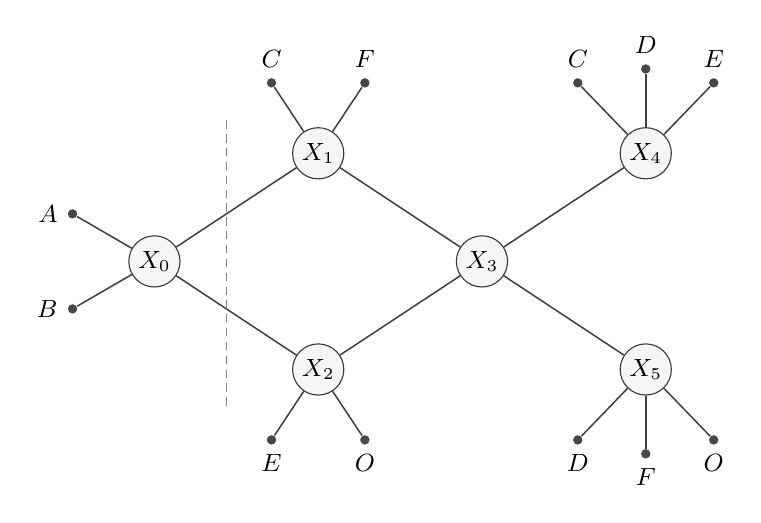
\begin{tikzpicture}[
  x=1.04cm,y=1.04cm,
  bulk/.style={circle,draw=black!78,fill=black!4,inner sep=1.6pt,
               minimum size=6.5mm,font=\small},
  port/.style={circle,fill=black!72,inner sep=1.2pt},
  every edge/.style={draw=black!75,line width=0.55pt}
]
  \node[bulk] (x0) at (0,0) {$X_0$};
  \node[bulk] (x1) at (2,1.32) {$X_1$};
  \node[bulk] (x2) at (2,-1.32) {$X_2$};
  \node[bulk] (x3) at (4,0) {$X_3$};
  \node[bulk] (x4) at (6,1.32) {$X_4$};
  \node[bulk] (x5) at (6,-1.32) {$X_5$};
  \path (x0) edge (x1) edge (x2)
        (x3) edge (x1) edge (x2) edge (x4) edge (x5);
  \foreach \id/\xx/\yy/\lab/\at/\pos in {
    a/-1.0/0.58/A/x0/left,b/-1.0/-0.58/B/x0/left,
    c1/1.43/2.18/C/x1/above,f1/2.57/2.18/F/x1/above,
    e2/1.43/-2.18/E/x2/below,o2/2.57/-2.18/O/x2/below,
    c4/5.17/2.18/C/x4/above,d4/6.0/2.35/D/x4/above,e4/6.83/2.18/E/x4/above,
    d5/5.17/-2.18/D/x5/below,f5/6.0/-2.35/F/x5/below,o5/6.83/-2.18/O/x5/below}
  {
    \node[port,label={\pos:\small\(\lab\)}] (\id) at (\xx,\yy) {};
    \path (\id) edge (\at);
  }
  \draw[densely dashed,black!48] (0.88,-1.76) -- (0.88,1.76);
\end{tikzpicture}
\caption{Unit witness for ray \(110\) with separate leaves of the same
color. The dashed line selects an optimal \(AB\)-shore. Its two
crossing edges meet \(X_1\) and \(X_2\) on the right.}
\label{fig:ray110}
\end{figure}

\begin{theorem}[A sharp family from ray \(110\)]
\label{thm:chain}
For each \(k\geq1\) there is a genuine \(\SAC\)- and \(\HEC\)-extreme
vector \(u_k\) on \(5k+1\) named parties with \(\gamma(u_k)=k\).
Every realization contains \(k\) pairwise vertex-disjoint cycles.
There is a rigid connected unit realization with four-valent bulk
vertices. At every designated prefix--suffix partition in a connected
positive realization \(G\), every optimal separating cut has at most
\(\beta(G)-k+1\) edges.
\end{theorem}

\begin{proof}
Relabel \(k\) copies of the witness independently. Splice port \(B\)
of each copy to port \(A\) of the next. The unused ports remain unit
leaves, so all splices have matched singleton one. Corollary~\ref{cor:rigid}
gives SAC extremality and rigidity, and connectedness gives genuineness.
There are \(7k-2(k-1)=5k+2\) colors including a chosen purifier.
The graph has \(6k\) bulk vertices, \(10k+2\) leaves, and \(17k+1\)
edges, so its cycle rank is \(k\).

In an arbitrary realization, slice at the color partition of the last
splice. The two factors are the shorter chain and the seed. The seed
requires a cycle by Appendix~\ref{app:seed}. Repeating the slicing
lemma gives \(k\) cycles in disjoint induced vertex sets. An added
port leaf lies on no cycle, so all these cycles belong to the original
graph. This proves the sharp minimum without an assumption on the
size, topology, or terminal multiplicities of the competing realization.

At any designated prefix--suffix partition the two projections are
chains whose minimum ranks add to \(k\). Theorem~\ref{thm:seam} gives
the final bound. At minimum rank, the least optimal prefix shores
are nested by cut submodularity and have one crossing edge each.
The bridges are distinct because their color partitions differ.
Removing them separates \(k\) connected pieces, and restoring port
leaves recovers one seed vector on each by repeated application of
Lemma~\ref{lem:slice}. Each piece then has cycle rank one.
\end{proof}

The explicit realization also gives a minimally degenerate fine lift.
Assign a distinct color to every terminal leaf. The fine weight cell
has the same scaling span as the coarse cell because all coarse
min-cut problems occur among the fine ones. The fine vector is SAC
extreme by the even-degree unit-leaf lemma proved in
Appendix~\ref{app:even}. This ties the original weight-cell and SAC
constructions to the representation-independent lower bound.

The edge-count bound can be sharp above the minimum rank. For two
blocks, double the capacities and replace their capacity-two bridge
by two internally disjoint paths of two unit edges each. For fixed
endpoint bits the two paths have total minimized cost zero or two,
so the entropy vector is twice the original. The graph has one excess
cycle and an optimal seam crossing two edges. Each of the four choices
of sides of the two new internal vertices at that seam gives exact
factor slices with two port leaves.

\section{The interface cost of ray 110}
\label{sec:interface}

Consider \(AB\mid CDEFO\) in Figure~\ref{fig:ray110}. The shore
\(\{A,B,X_0\}\) has cost two, which is the minimum. In fact, if \(X_0\)
is outside, the \(A,B\) leaf edges cost two. If \(X_0\) is inside,
each of the two paths to an unselected leaf through \(X_1,X_2\) must
be cut. Slicing along this shore yields two trees. The left factor \(s\)
is a three-color star with arm capacities \(1,1,2\) after combining
its two port leaves at \(X_0\). The right factor \(t\) has two
unit leaves of port color \(q\), one at \(X_1\) and the other at \(X_2\).

The two factors splice back to \(\ray\) with interface capacity two.
To see the entropy identity directly, fix the terminal bits
\(\alpha,\eta\) at \(A,B\), and fix a side bit \(\varepsilon\) for
the port of the left factor. Its minimum is
\[
 \min_{\zeta\in\{0,1\}}
 \bigl(|\alpha-\zeta|+|\eta-\zeta|+2|\zeta-\varepsilon|\bigr)
 =|\alpha-\varepsilon|+|\eta-\varepsilon|.
\]
The inequality that proves this equality is just the triangle
inequality for the two leaf terms. In the right slice the port bit
\(\varepsilon\) contributes
\(|x_1-\varepsilon|+|x_2-\varepsilon|\), where \(x_i\) is the side of
\(X_i\). Minimizing the sum over \(\varepsilon\) and over the right
bulk bits is exactly the original minimum with \(X_0\) free.
This is~\eqref{eq:branches}, so the bridge criterion holds even
though the displayed witness uses two edges at this cut.

\begin{theorem}[A marked color can force a cycle]
\label{thm:portcost}
For these factors, \(\gamma(s)=\gamma_p(s)=\gamma(t)=0\), while
\(\gamma_q(t)=1\). In particular,
\(\gamma(s\star t)=1>\gamma(s)+\gamma(t)\).
\end{theorem}

\begin{proof}
The three zeros are witnessed by the trees just described. If the
right factor admitted a forest with \(q\) occurring once, port
normalization would supply a capacity-two pendant port at the same
cycle rank. Splicing it to the left tree would realize \(\ray\) by a
forest, contradicting Appendix~\ref{app:seed}. For the upper bound,
identify the two \(q\) leaves in the right tree. The identification
preserves its entropy because those leaves already had a common
prescribed side. It reduces the vertex count by one at fixed edge
and component counts, producing one independent cycle. If a pendant
port is desired, Lemma~\ref{lem:port} adds it without another cycle.
\end{proof}

The same example shows that extremality need not descend to the
factors. Rational elimination gives their PMI dimensions as two and
five. Matching the singleton leaves dimension six, and the equations
from the 40 tied mixed masks have rank five on that space. This gives
the one-dimensional PMI of the splice by Theorem~\ref{thm:linear}.
For the pendant-normalized models, the two factor weight cells have
span dimensions two and one, whereas the splice's span has dimension
one. The counts and ranks can be regenerated from the edge list in the
reproduction archive.

\section{Nonclosure for every fixed cycle-rank bound}
\label{sec:limit}

For a fixed color set \(P\) and integer \(b\geq0\), let \(\mathcal G_b(P)\)
be the graph entropy vectors with \(\gamma(u)\leq b\). We will use a
shared purifier rather than the bridge splice of
Theorem~\ref{thm:chain}. This makes it possible to combine connected
tree approximants without introducing any cycles.

\begin{theorem}[Nonclosure at fixed cycle budget]
\label{thm:nonclosed}
For every \(b\geq0\), on a color set of \(6(b+1)\) named parties and one
purifier, there is a genuine vector in
\[
 \bigl(\mathcal G_{b+1}(P)\setminus\mathcal G_b(P)\bigr)
 \ \cap\ \overline{\mathcal G_0(P)}.
\]
The approximants can all be realized by connected positive trees.
\end{theorem}

\begin{proof}
Put \(k=b+1\). Use pairwise disjoint six-color blocks \(A_1,\ldots,A_k\)
and one common purifier \(O\). Define \(v_k\) on masks omitting \(O\)
by
\begin{equation}
 v_k(X)=\sum_{i=1}^k \ray(X\cap A_i),
 \label{eq:sum}
\end{equation}
with the colors in each summand relabeled in \(A_i\). Extend by purity.
The vector is genuine because every nonempty mask omitting \(O\)
intersects a block. Identifying one \(O\)-colored vertex from each
unit witness realizes~\eqref{eq:sum} in a connected graph of cycle
rank \(k\). The shared vertex is pinned, so the cut problems still
optimize independently.

For the lower bound in an arbitrary realization, take the
inclusion-least optimal shores \(U_i\) for \(A_i\). Such a shore exists
because the intersection of two optimal shores for the same mask is
again optimal by submodularity. The shores \(U_i\) are pairwise
disjoint. Indeed, for \(i\ne j\), cut posimodularity makes the
differences \(U_i\setminus U_j\) and \(U_j\setminus U_i\) optimal for
their respective masks, because the masks are disjoint. Leastness
excludes an overlap. Slicing each \(U_i\), with its complement grouped
into the port color, recovers \(\ray\) by~\eqref{eq:sum} and
Lemma~\ref{lem:slice}. Thus each induced shore contains a cycle.
This proves \(\gamma(v_k)=k\).

To approximate one copy of \(\ray\), take \(L\) sheets of its
boundary-split unicyclic witness. Lift every edge within each sheet
except one edge of the bulk cycle, which joins each sheet to the next
cyclically. The resulting graph is a connected cycle of length \(4L\)
with trees attached. Its entropy is exactly \(L\ray\).
For the upper bound, copy a base optimum. For the lower bound, for
each base vertex \(v\) let \(x_v\) be the fraction of its copies on
the chosen shore. The lift of each base edge \(vw\) contributes at
least \(L|x_v-x_w|\) times its capacity, by the matching of its
endpoints. Thresholding the \(x_v\) at levels in \((0,1)\) and
integrating gives at least \(L\) times the base minimum, since the
boundary fractions are prescribed zeros and ones.

Delete one unit edge of the lifted cycle and divide every capacity by
\(L\). The result is a connected positive tree with vector \(S_L\)
satisfying \(0\leq\ray(X)-S_L(X)\leq1/L\) in every coordinate.
Use one such tree per block and identify one purifier vertex per tree
to a common \(O\)-colored vertex. This one-point union is still a tree.
Its entropy differs from \(v_k\) by at most \(k/L\) in sup norm, with
the exact sum property following from the pinned common vertex.
Taking \(L\) to infinity proves the claim.
\end{proof}

The extreme vectors \(u_k\) in Theorem~\ref{thm:chain} and the limits
\(v_k\) in Theorem~\ref{thm:nonclosed} use different compositions.
The first retains extremality and pins down the topology of
cycle-rank-minimal realizations. The second retains the connected
tree approximation while adding the lower bounds on cycle rank.

\section{Consequences for conjectures C1--C4}
\label{sec:conjectures}

We use the scope and numbering of \cite[Sec.~6.2]{hhr2022}. The bridge
construction supplies a family of examples. The universal lifting
argument needed for C1 and C2 is given in Appendix~\ref{app:universal}.

\paragraph{C1 and C2.}
Theorem~\ref{thm:universal-lift} starts with an arbitrary genuine
\(\HEC\) extreme ray. It produces a finite fine-graining on the same
underlying graph as its coarse representative. The coarse and fine
weight cells have the same linear span, and the fine min-cut subspace
equals its nowhere-zero PMI. This is C1. The fine vector generates a
\(\SAC\) extreme ray and its color projection recovers the prescribed
coarse vector after normalization, which proves C2. The appendix also
handles C2 for rays with spectator colors.

\paragraph{C3.}
Lemma~\ref{lem:seed} verifies that \(\ray\) generates a genuine
\(\HEC\) extreme ray. The same lemma excludes every finite tree
realization with repeated terminal colors and nonnegative real
capacities. Thus \(\ray\) disproves C3.

\begin{corollary}[Counterexample to C4]
\label{cor:c4}
Let \(G_*\) be the unit witness in Figure~\ref{fig:ray110}, and
let \(\mathfrak m_*\) be its min-cut structure. Then
\(\MC(G_*,\mathfrak m_*)=\mathbb R\ray\).
No tree min-cut structure has this subspace.
\end{corollary}

\begin{proof}
The coarse tied-cut rows at the unit witness have rank 17 in
18 edge coordinates by Lemma~\ref{lem:seed}, so its weight cell
consists of positive uniform rescalings. Its entropy image spans
\(\mathbb R\ray\). If a tree min-cut structure had this same
span, some nonzero entropy vector in its cell would belong to
that line. Nonnegativity would make it a positive multiple of
\(\ray\). Rescaling the tree would realize \(\ray\), contradicting
Lemma~\ref{lem:seed}.
\end{proof}

Corollary~\ref{cor:c4} concerns equality of min-cut subspaces, the
claim in \cite[Eq.~(6.11)]{hhr2022}. Theorem~\ref{thm:nonclosed}
concerns limits of entropy vectors under a fixed cycle-rank bound.

Ju and Czech~\cite[Secs.~IV--V and App.~A]{juczech2026} prove that the
mutual information of any pair of colors in a finite tree graph is
Bell-extractable. Their Figure~1 gives a seven-party extreme ray with
\(I(A:B)=2\) for which Bell extraction fails. This refutes C3 and
therefore C4, by the implication in \cite[Sec.~6.2]{hhr2022}.
For the six-party ray \(\ray\), the seed coordinates give
\(I(i:j)=S_i+S_j-S_{ij}=0\) for every pair of distinct singleton colors
\(i,j\), including the purifier. The forest-exclusion certificate
establishes the obstruction for this ray. The bridge and slicing
results then propagate it to the families with specified minimum
cycle rank.

\section*{Reproducibility}
\addcontentsline{toc}{section}{Reproducibility}

The \href{https://github.com/LeoLam233/holographic-entropy-bridges}
{companion repository} contains the weighted edge data, the ray-\(110\)
forest-exclusion certificate, and verification commands for Python
3.10 or later. The forest-exclusion checks use the standard library.
The C1 splitting checks and the bridge example verifier use NumPy and
SciPy. The latter compares direct bulk-assignment enumeration with
integer max flow on all \(4096\) masks of the two-block example. It
checks rank \(34\) for the tied cut differences on 35 edge coordinates
and rank \(2046\) for the tight subadditivity rows on \(2047\) pure
entropy coordinates. For the marked-port example it checks the PMI and
weight-cell dimensions, the 40 tied branches and their additional rank.

\appendix
\section{The ray-110 seed certificate}
\label{app:seed}

This appendix states the scope and logical steps of the seed used in
the applications. The companion certificate supplies the finite
arithmetic, together with a detailed proof note and an independently
executable verifier. In particular, the forest exclusion uses a
finite-state induction, rather than an enumeration of trees up to a
chosen size.

\begin{lemma}[Seed properties]
\label{lem:seed}
The six-party ray \(110\) is genuine and SAC extreme. The unit witness
in Figure~\ref{fig:ray110} has a rigid coarse weight cell. No finite
weighted forest with repeated boundary colors realizes this vector,
even allowing arbitrary nonnegative real capacities.
\end{lemma}

\begin{proof}[Proof with the companion certificate]
The edge list and target coordinates come from the archived graph
data~\cite{fletcher} and the ray catalogue~\cite{hhr2025}. Exhaustive
cut enumeration and integer max flow agree on the 128 masks.
All proper nonempty coordinates are positive. Over the prime field
of order 1009, the tight subadditivity rows have rank \(62\) in
dimension \(63\), and the coarse tied-cut differences have rank \(17\)
on 18 edge coordinates. These are also the real ranks, since the
nonzero entropy vector and the all-one weight vector, respectively,
belong to the two kernels. Splitting terminal incidences into
same-color leaves preserves the coarse cut problems for arbitrary
weights and hence preserves the weight-cell span.

Suppose a forest realized the vector. Delete zero-capacity edges.
Each nonzero connected component realizes a positive multiple of
the vector by extremality. Rescaling such a component gives a
positive tree with the original entropy vector. Among all such trees,
minimize first the number of vertices and then the number of
uncolored vertices.

For each color mask \(I\), let \(U_I\) be the least optimal shore.
A vertex has signature \(I\mapsto \mathbf 1_{U_I}(v)\). Cut
submodularity makes these signatures monotone under inclusion.
Purity makes the largest optimal \(I\)-shore the complement of the
least optimal \(I^c\)-shore. Whenever the entropy submodularity
inequality for \(I,J\) is tight, uncrossing makes the least union
shore equal to \(U_I\cup U_J\). These facts give the Boolean signature
constraints. If an uncolored vertex is forced inside only on masks
containing some one color, it can be assigned that color while
preserving an optimal shore for each mask. Minimality removes this
case. Likewise, if every mask has an optimum putting the two
endpoints of an edge on the same side, that edge can be contracted
while preserving every entropy. Whether such an optimum exists can
be read from the least and greatest optimal shores. Finally, tight cut
submodularity and posimodularity forbid any edge type with a positive
contribution to the corresponding uncrossing slack. The finite
checks give 347 signatures before the pinning reduction, then
190 signatures and 226 candidate edge types.

Root a branch at each directed tree edge, looking away from its
parent. The branch state bounds the masks for which its root can
reach a terminal along a same-side path within the branch. The
terminal base case is immediate, and a nonterminal's possible
reachability is bounded by the same-side child states. If its parent
edge crosses a least optimal shore, the root side must reach a
terminal within the branch. Otherwise a terminal-free component
could be flipped and strictly decrease the cut. For an additional
capacity test, flip the root with its same-side child components
that fail to reach any terminal. The cost change is bounded above by
the sum of the signed parent and crossing edges and the same-side
child edges allowed by the reachability bounds. This upper bound
must be nonnegative, and is strictly positive if the root was on
the least shore. The certificate verifies the state closure and
excludes all other directed types by these tests and nonnegative
rational combinations of their capacity rows. Induction from the
leaves applies to every finite branch depth. The surviving undirected
support has 34 edge types in two layers, related by exchanging
colors \(E,F\).

On this support, aggregate the capacities by edge type. The entropy
equalities and nonnegative costs of flipping sets of uncolored
types force 18 aggregate flip rows to vanish. The supplied rational
identities certify this implication, and the combined system has
rank 33 on 34 edge types. The nonnegative solutions are therefore
convex combinations of the two unit layers. In each layer, tight
single-type flips force equal incident type capacities at each
occurrence of types \(X_1,X_2,X_4,X_5\), with the analogous statement
for the exchanged layer. Tight flips of each connected layer
component then force a component incident to the shared type \(X_0\)
to have at least two such incidences. At an occurrence of \(X_0\)
with only one bulk edge of capacity \(d>0\), two least-cut
optimality rows on the capacities to colors \(A,B\) would imply
\(w_A-w_B-d\geq0\) and \(w_B-w_A-d\geq0\), an impossibility.

Delete colored vertices, contract the layer components, and discard
isolated vertices. A layer has positive total capacity, so the
remaining graph is nonempty. The certified local and component
equalities imply minimum degree at least two, whereas these
operations on a finite tree produce a forest. This contradiction
excludes the putative realization. The companion verifier
reconstructs the signature closure, checks the aggregate equalities
over the rationals, and verifies the degree implications.
\end{proof}

\section{SAC extremality for an even-degree unit graph}
\label{app:even}

\begin{lemma}
\label{lem:even-lift}
A connected unit-capacity graph with degree-one terminals of distinct
colors and even bulk degrees generates an extreme ray of the SAC.
\end{lemma}

\begin{proof}
Every singleton entropy is one. Pair bulk incidences to partition
edges into trails connecting terminal pairs and closed trails. To
require a chosen pair \(i,j\), first delete a simple path between
them and pair the remaining incidences. A transversal taking one
terminal of each pair has entropy equal to its number of terminals
by the disjoint trail lower bound and the pendant-cut upper bound.
The same holds for its complement. Both statements are tight
subadditivity equations. Comparing transversals differing only in
the choice between \(i,j\) proves that their singleton directions
agree on the PMI. Thus all singleton directions agree.

For an arbitrary terminal mask \(X\), take an optimal bulk side \(U\)
and let \(B(U)\) be the terminals whose neighbors are in \(U\).
Toggling a terminal disagreeing with \(U\) lowers the chosen cut cost
by one and lowers every competing cut cost by at most one. Each
toggle therefore preserves optimality of \(U\) and gives a tight
singleton subadditivity equality, using purity when needed.
Thus all PMI directions \(a\) obey
\[
 a_X=a_{B(U)}+\sum_{i\in X\triangle B(U)}a_{\{i\}}.
\]
At \(B(U)\), use integral maximum flow to pair terminals across
the bulk cut. The paths consume its crossing edges exactly once.
Pair the remaining terminals by trails on each side, using the
remaining even bulk degrees. Take a transversal \(Y\) that uses the
\(B(U)\)-side endpoint of every crossing path and one endpoint of
every remaining trail. The bulk side \(U\) realizes its locked
transversal minimum. Therefore \(a_Y\) is a sum of singleton
directions and the toggle formula at \(Y\) determines \(a_{B(U)}\).
Every coordinate is now determined by the common singleton
direction. The single-edge case follows directly from purity.
\end{proof}

\section{A rigid fine-graining for every extreme ray}
\label{app:universal}

\begin{theorem}
\label{thm:universal-lift}
Let \(s\) generate a genuine extreme ray of the static \(\HEC\).
There is a finite connected graph with unit edge capacities, terminal
leaves, and four-valent bulk vertices that realizes a positive multiple
of \(s\) with its coarse colors. Giving each leaf a distinct fine
color yields a vector \(r\) with
\[
 \operatorname{span}W_{\rm fine}
 =\operatorname{span}W_{\rm coarse}=\mathbb R\mathbf 1,
 \qquad \MC_{\rm fine}=P(r)=\mathbb Rr.
\]
All proper nonempty fine entropies are positive. A common rescaling
gives a graph-realizable SAC extreme vector whose color projection
equals \(s\).
\end{theorem}

\begin{proof}
\emph{Unit capacities and even bulk degrees.}
Take any finite graph realizing \(s\) and delete zero-capacity edges.
Its weight cell is relatively open in a linear space given by
integer cut-difference rows, so a nearby point of the cell has positive
rational capacities. The entropy map is linear on the cell. For the
direction to the rational point, a small step in the opposite direction
is still in the cell. Extremality of \(s\) forces the two image vectors
onto its ray, and the nearby rational point has nonzero entropy.

Clear denominators and multiply by two. Replace each resulting edge
capacity by that many parallel unit edges. Separate the incidences of
each colored vertex into leaves carrying its original color. The same
terminal bits are prescribed in every coarse cut, so this preserves
the scaled coarse entropy. Each bulk vertex now has even degree.
Discard loops and isolated bulk vertices. A degree-two bulk vertex
can be suppressed by replacing its two unit edges by one unit edge
between its neighbors. The resulting edge has the same minimum cost
conditional on the two neighbor bits. If the neighbors coincide,
the resulting loop can be discarded.

\emph{Four-valent replacement.}
Replace a bulk vertex of degree \(2m>4\) by a network with \(2m\)
ports. Use \(m\) edge-disjoint wires with two ports per wire. Make
each pair of wires meet at one shared vertex, and let each wire
visit its crossing vertices in any order. These new vertices all
have degree four. For any fixed port assignment, a cut isolating
the smaller set of ports costs at most its size. For the matching
lower bound, keep the wires with opposite-side ends as paths.
Pair as many wires having two selected ends with wires having two
unselected ends as possible, using each wire at most once. At the
shared vertex of each pair, reconnect their four halves into two
paths with opposite-side ends. The resulting paths are edge disjoint.
Their count is the size of the smaller port set. The network
therefore has the same port cut function as the unit star on the
same ports.

Attach the original incident edges to the ports. The conditional
minimum over the new network can be computed with the equivalent
star in its place, followed by minimization over the port bits.
Each star arm and attached edge is a two-edge unit path in series,
so its minimized cost is that of the original incident edge.
Suppress the degree-two ports in the new network. Repeating this
replacement gives a unit graph whose bulk degrees are four, after
the degree-two and loop simplifications.

\emph{Split off a missing balanced partition.}
For any fixed coarse mask and any feasible shore \(U\),
\[
 |\delta_G U|\equiv \sum_{v\in U}\deg(v)
 \equiv |U\cap T|\pmod 2,
\]
where \(T\) is the set of terminal leaves. This parity is the same
for every feasible shore of the mask. At a four-valent vertex
label the four incident edge ends \(1,2,3,4\). A balanced partition
occurs when the neighbor bits are constant within each pair of
some two-pair partition and opposite between the pairs. Suppose
one of the three such partitions never occurs in a coarse optimum,
for any mask. Remove the vertex and join the neighbors in the
two pairs of the missing partition by unit edges.

For fixed bits away from the removed vertex, the old locally
minimized cost at that vertex is \(\min(h,4-h)\), where \(h\) is
the number of selected neighbor incidences. The new cost is the
number of opposite-bit pairs. It is the same except at the
specified balanced pattern, where it is lower by two. The new
minimum is at most the old one. If it were strictly smaller,
lifting that assignment and minimizing at the old vertex would
give a feasible old cut less than two above the old minimum.
Parity would make it an old optimum, which would have the
missing pattern. This contradiction proves exact preservation
of every coarse cut value. The argument uses the critical-cut
parity principle for splitting off in inner-Eulerian
networks~\cite{hirai2010}.

After each step remove loops and suppress any degree-two bulk
vertices. Terminal degrees stay one, bulk degrees stay even and
at most four, and the number of bulk vertices decreases. On
termination all three patterns occur in coarse optima at every
remaining bulk vertex. The graph may have become disconnected,
but its total coarse entropy vector is unchanged. Each nonzero
component realizes a positive multiple of \(s\) by extremality.
Keep one such component. Genuineness guarantees that it contains
all coarse colors. The optimal shores restrict to component
optima, so all three local witnesses survive. Parallel edges
would share a neighbor bit at a bulk vertex and preclude one of
the patterns. Thus the retained graph is simple.

\emph{Rigidity and the fine lift.}
At each retained bulk vertex, flipping that vertex alone in the
three witnessed optima gives ties with the corresponding
opposite shore choices. The three resulting equations on its
incident capacities are
\[
 w_1+w_2=w_3+w_4,\qquad w_1+w_3=w_2+w_4,\qquad
 w_1+w_4=w_2+w_3.
\]
They force all four weights equal. Connectivity and the pendant
boundary propagate equality to every edge. If there is no bulk
vertex, the connected component is a single terminal edge and
its weight space already has dimension one. Positive rescaling
preserves the coarse structure, so the coarse span is exactly
\(\mathbb R\mathbf 1\).

After giving all leaves distinct colors, the coarse masks are
among the fine masks, so the fine span is contained in the coarse
span and contains the same scaling direction. The fine min-cut
subspace is \(\mathbb Rr\), which equals \(P(r)\) by
Lemma~\ref{lem:even-lift}. Connectivity and positive capacities
give positivity of every proper nonempty coordinate. Grouping
the fine leaves by their inherited colors reproduces the coarse
vector. A common scaling fixes its normalization.
\end{proof}

For C2 on a ray with spectator colors, the same reduction yields
a connected nonzero component proportional to the prescribed ray.
Any original color absent in it has zero singleton entropy.
Adjoin one isolated fine terminal for each missing coarse color
and assign it that color in the projection. For such a fine
terminal \(p\), the tight SA row between \(p\) and its complement
forces the \(p\)-singleton direction to vanish, and the tight
row between \(p\) and any disjoint mask forces the coordinates
with and without \(p\) to agree. Thus the spectator extension
preserves one-dimensionality of the fine PMI and gives the
desired full color projection.

\begin{thebibliography}{9}
\setlength{\itemsep}{0.26em}
\bibitem{bao2015}
N.~Bao, S.~Nezami, H.~Ooguri, B.~Stoica, J.~Sully, and M.~Walter,
\emph{The holographic entropy cone},
JHEP \textbf{09} (2015) 130.
\href{https://arxiv.org/abs/1505.07839}{arXiv:1505.07839}.

\bibitem{hhr2022}
S.~Hern\'andez-Cuenca, V.~E.~Hubeny, and M.~Rota,
\emph{The holographic entropy cone from marginal independence},
JHEP \textbf{09} (2022) 190.
\href{https://arxiv.org/abs/2204.00075}{arXiv:2204.00075}.

\bibitem{hhj2024}
S.~Hern\'andez-Cuenca, V.~E.~Hubeny, and H.~F.~Jia,
\emph{Holographic entropy inequalities and multipartite entanglement},
JHEP \textbf{08} (2024) 238.
\href{https://arxiv.org/abs/2309.06296}{arXiv:2309.06296}.

\bibitem{hhr2025}
T.~He, V.~E.~Hubeny, and M.~Rota,
\emph{Algorithmic construction of SSA-compatible extreme rays of the
subadditivity cone and the \(N=6\) solution},
\href{https://arxiv.org/abs/2412.15364}{arXiv:2412.15364}.

\bibitem{fletcher}
A.~M.~Fletcher,
\emph{Independent exact graph realizations of holographic mystery
rays 110, 145, and 168}, version 1.0.0,
Zenodo (2026).
\href{https://doi.org/10.5281/zenodo.22020364}{doi:10.5281/zenodo.22020364}.

\bibitem{juczech2026}
X.-X.~Ju and B.~Czech,
\emph{Not all holographic entropy inequalities are free of area law
ultraviolet divergences},
\href{https://arxiv.org/abs/2611.21726v1}{arXiv:2611.21726v1} (2026).

\bibitem{hirai2010}
H.~Hirai, \emph{A note on multiflow locking theorem},
J. Oper. Res. Soc. Japan \textbf{53} (2010), 149--156.
\href{https://doi.org/10.15807/jorsj.53.149}{doi:10.15807/jorsj.53.149}.
\end{thebibliography}

\end{document}
